The ongoing digital transformation of science, industry, and society has progressively changed both the role assigned to data and the software infrastructures used to manage it. Early information systems were primarily concerned with recording and managing operational events. As analytical techniques and computational infrastructures matured, these records became the basis for information, knowledge, and decision support. Subsequently, the widespread deployment of sensors, connected devices, distributed computing, and streaming infrastructures extended the scope of digital systems from enterprise processes to continuously monitored physical environments.

This evolution can therefore be considered from two complementary and increasingly intertwined perspectives. The first concerns the changing role and value attributed to data: from a record of an event, to information about that event, to knowledge derived from collections of observations, and ultimately to a basis for decision and action. The second concerns the evolution of the computational infrastructures required to support these transformations: from transactional information systems and analytical warehouses to distributed cloud data platforms, continuous processing infrastructures, and cyber-physical systems.

The two trajectories are not independent. Each new class of systems has emerged in response to new requirements concerning the scale, variety, timeliness, and use of data, while the increasing availability of data has, in turn, enabled new computational capabilities. The history of digital systems can therefore be interpreted not simply as a succession of technologies, but as an intertwined evolution in which changes in the role of data and changes in computing infrastructures continuously influence one another.

These trajectories increasingly converge as digital systems become capable of continuously observing and interacting with physical processes. Data is no longer only a record of what has happened, but a basis for understanding what is happening, estimating what may happen next, and supporting decisions concerning what should happen. This progression provides the technological and conceptual background against which the recent proliferation of Digital Twin systems and artificial intelligence should be understood.

This chapter traces these developments as a foundation for the remainder of the thesis. It focuses on the evolution of data and of the computational infrastructures surrounding it, with particular attention to the changing requirements for data management that accompanied each stage.

% =========================================================================
\section{Digitalization -- From Data to Wisdom}
\label{sec:digitalization_data_knowledge}
% =========================================================================

The history of digital information systems can be interpreted as a progressive transformation in the role of data. In the earliest stages of electronic data processing, computational systems were primarily employed to automate repetitive calculations and to maintain records of organizational activities. Financial transactions, inventory movements, administrative records, and other operational events were represented as structured data whose primary purpose was to document the state of an organization and support the execution of its processes.

The introduction of the relational data model provided a rigorous foundation for the management of such information. Relational Database Management Systems, together with Online Transaction Processing (OLTP), established an architectural paradigm centered on structured schemas, transactional consistency, integrity constraints, and reliable updates \cite{codd1970,gray1992}. At this stage, the requirements imposed on data management were therefore primarily concerned with correctness, consistency, persistence, and efficient access to operational data. Data was mainly an operational asset: its value depended on its ability to faithfully represent the state of the processes that generated it.

As organizations accumulated increasing amounts of operational data, a new opportunity emerged. Data generated by individual transactions could also be exploited beyond the process in which it had originally been produced. Organizations began to integrate data across processes and over time in order to obtain aggregated indicators, identify historical patterns, compare operational states, and support planning and management decisions. This shift motivated the development of Data Warehousing and Business Intelligence architectures, which enabled integrated and multidimensional analysis of historical organizational data \cite{inmon1992,kimball2002}.

The role of data consequently expanded from operational record to analytical resource. Transactional systems were primarily concerned with faithfully recording the state of operational processes, whereas analytical infrastructures enabled organizations to examine trends, correlations, historical behaviour, and organizational performance across time and across processes. The change was not only a change in how data was used; it also introduced new requirements for how data had to be managed. Data originating from multiple operational systems had to be integrated, consolidated, transformed, and organized according to analytical purposes.

A useful conceptual representation of this progression is provided by the Data--Information--Knowledge--Wisdom (DIKW) framework (\Cref{fig:dikw}). Widely discussed as a conceptual model of increasing levels of meaning, it distinguishes between data as observations, information as contextualized and organized data, knowledge as the result of identifying relationships and patterns, and wisdom as the informed application of knowledge to judgement and decision making \cite{ackoff1989,rowley2007}.

\begin{figure}[htbp]
    \centering
    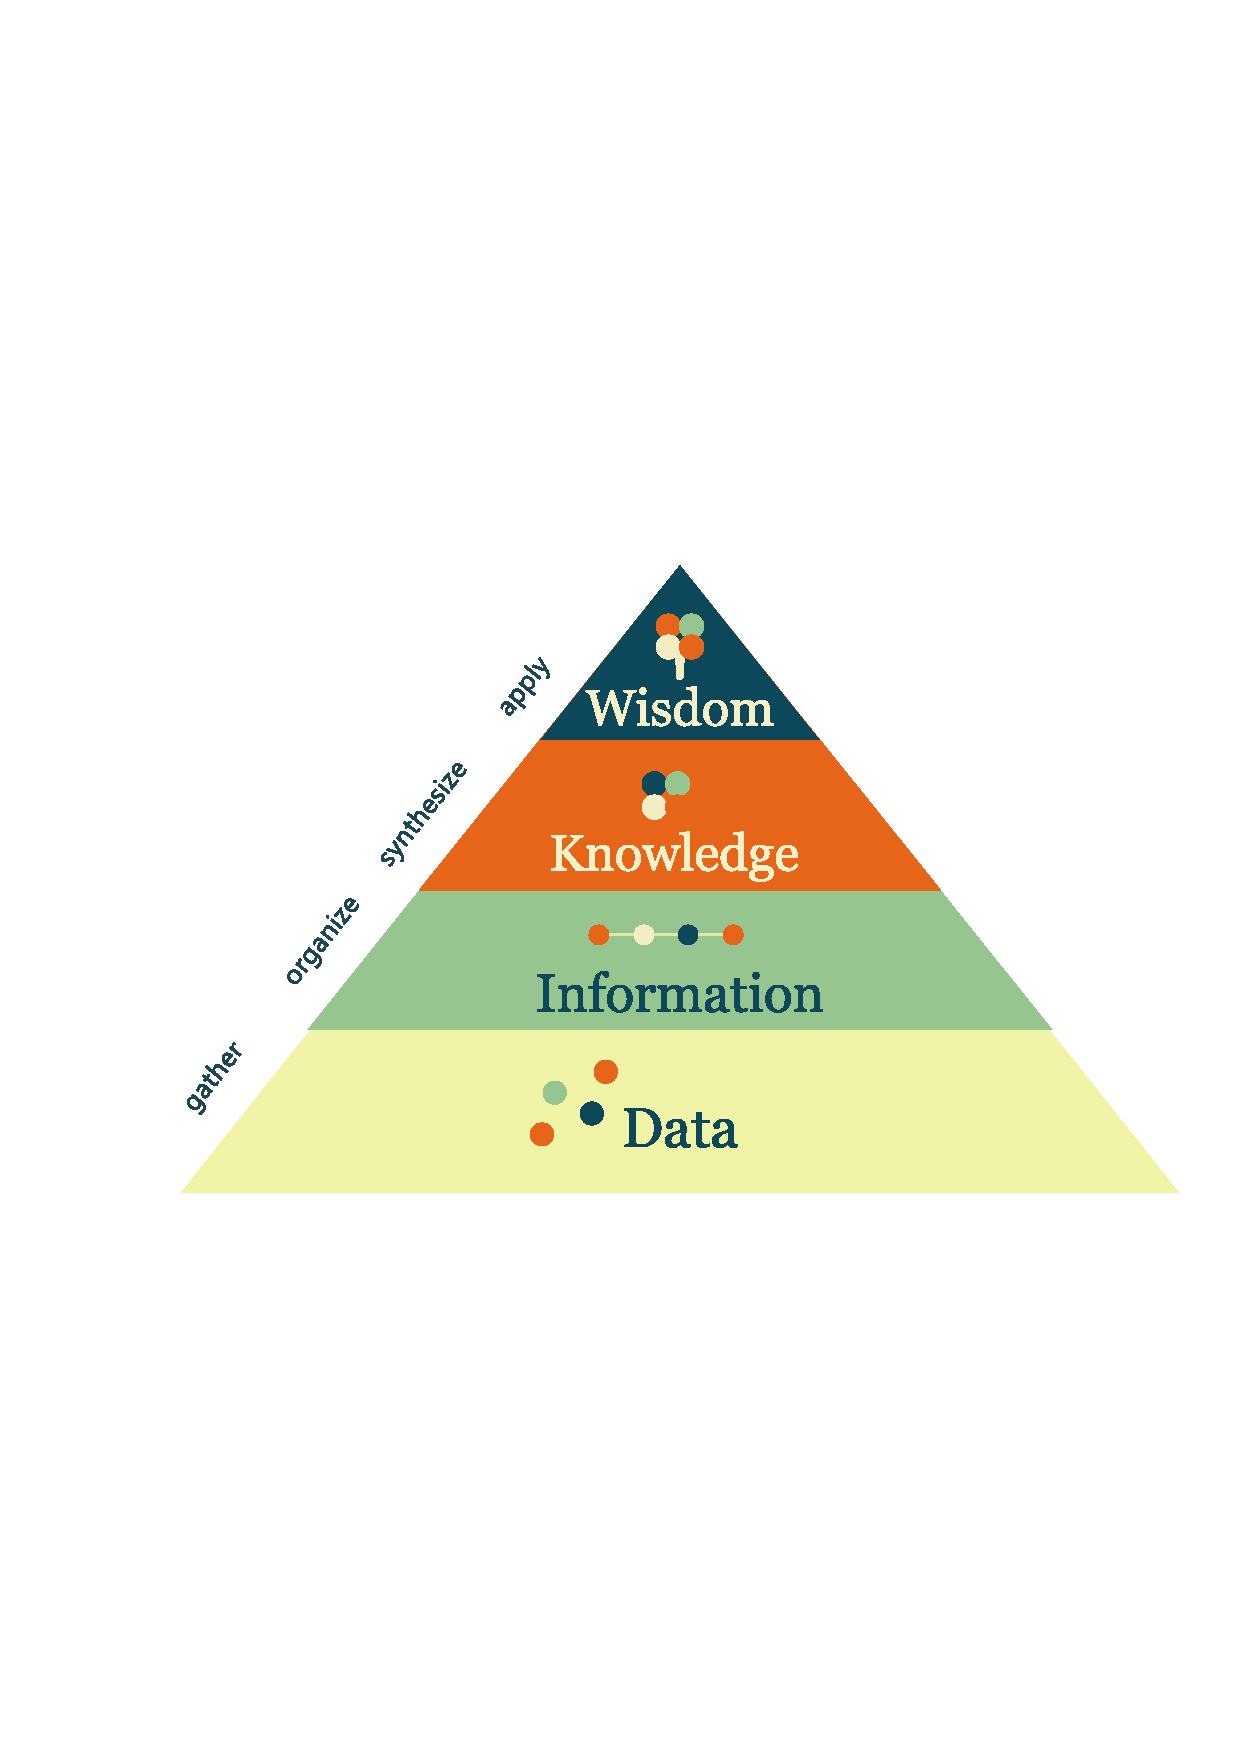
\includegraphics[trim=0 260pt 0 260pt, clip, width=0.75\textwidth]{parts/foundations/images/dikw_pyramid.pdf}
    \caption{Conceptual representation of DIKW pyramid.}
    \label{fig:dikw}
\end{figure}


The relevance of this framework in the context of digitalization lies less in the existence of a strict hierarchy than in the progressive transformation it emphasizes. The increasing value of data derives from the ability to move beyond its mere collection and towards its interpretation and use. Operational databases provide the means to capture observations reliably; analytical infrastructures organize and contextualize them; analytical methods extract patterns and models; and decision-support mechanisms make the resulting knowledge useful for planning and action.

This evolution also changed the requirements imposed on the infrastructures supporting data processing. As long as the principal objective was the reliable recording of operational events, relatively stable schemas and transaction-oriented workloads were sufficient. As data began to be integrated across systems and analyzed historically, systems had to support larger datasets, increasingly complex queries, heterogeneous sources, and transformations between operational and analytical representations.

The growing diversity of digital sources further amplified these requirements. Web applications, distributed software systems, multimedia repositories, machine logs, and eventually sensor infrastructures generated data with substantially greater volume and variety, often without the rigid structures traditionally associated with transactional systems. Data management therefore progressively moved beyond centralized relational databases towards scalable distributed infrastructures capable of storing and processing heterogeneous, semi-structured collections of data.

NoSQL solutions, data lakes and big data platforms emerged in response to these requirements, providing mechanisms for the large-scale storage and distributed processing of heterogeneous data. Later data lakehouse architectures attempted to combine the flexibility of large-scale data storage with stronger transactional, performance, and governance capabilities. Across these developments, a common trend can be observed: as the amount and diversity of data increased, the computational infrastructure had to become increasingly capable of integrating and processing data that could no longer be treated as a small collection of homogeneous, stable records. Consequently, data management in terms of integration and governance became just as important, if not more so, than the ability to efficiently store and retrieve data.

At the same time, the temporal dimension of data became increasingly important. Traditional analytical workloads were predominantly retrospective. They aimed to explain historical behaviour, compare past states, and identify patterns in accumulated records. As digital systems began to generate data continuously, however, a new requirement emerged: information had to be processed while the underlying process was still unfolding.

Streaming architectures consequently introduced a complementary computational model in which data could be ingested, transformed, enriched, and analyzed continuously rather than exclusively through periodic batch execution. The evolution from batch-oriented to continuous processing reduced the temporal distance between the observation of an event and the computational response to it.

This change was particularly relevant for predictive analytics. Once historical data could be combined with statistical and machine-learning methods, information systems were no longer limited to describing what had happened. They could estimate future states, identify emerging conditions, forecast demand, predict failures, and support decisions under uncertainty. The analytical objective consequently shifted from retrospective description towards anticipation.

More recent advances in artificial intelligence extend this trajectory further. Large-scale machine-learning systems can derive increasingly complex representations and predictions from heterogeneous data, while generative AI systems can synthesize information and interact with it through increasingly flexible interfaces. Emerging agentic AI systems further combine these capabilities with reasoning, planning, tool use, and execution. In this setting, data is not merely an input to an isolated analytical process. It becomes part of the context upon which a computational system bases decisions and actions.

The resulting progression can therefore be understood as a gradual reduction in the temporal and conceptual distance between data and action. Early information systems primarily recorded what had happened. Analytical systems transformed accumulated records into information and knowledge. Predictive systems increasingly estimated future states. Agentic AI systems can use such information to support decisions and, in some contexts, participate directly in their execution.

This progression continuously raises the requirements imposed on data management. The larger and more heterogeneous the datasets become, and the closer computation moves towards operational decision making, the more important it becomes that data can be obtained, processed, and interpreted in a timely and reliable manner. The relevant challenge is consequently no longer only how to store more data or process it faster, but how to manage data in ways that preserve its usefulness as it moves across increasingly heterogeneous computational environments.

While continuous data collection and storage techniques have become increasingly mature, the integration and governance of heterogeneous data needed to continuously derive meaningful knowledge and support timely action remain open challenges.

% =========================================================================
\section{From Information Systems to Cyber-Physical Systems}

\label{sec:dss_to_cps}

% =========================================================================

The evolution of data-intensive information systems was accompanied by a progressive expansion of the physical processes that could be digitally observed and computationally managed. Early information systems primarily operated on data generated by organizational activities and transactions. As analytical capabilities matured, these data were increasingly used to support monitoring, planning, and decision making through Business Intelligence, analytical models, and Decision Support Systems (DSS).

The emergence of the Internet of Things (IoT), together with advances in sensing technologies, embedded electronics, communication networks, and distributed computing, progressively extended this computational capability beyond traditional enterprise applications. Physical assets and environments could increasingly be equipped with sensors and connected devices capable of continuously acquiring and transmitting measurements about their state. In the context of Industry~4.0, this pervasive instrumentation became an important enabler of increasingly connected and data-intensive industrial environments.

The availability of continuous physical observations introduced a fundamental change in the relationship between information systems and the processes they represented. Instead of operating primarily on data generated by human or organizational activities, computational infrastructures could increasingly incorporate observations originating directly from the physical processes being monitored. These observations could then be integrated with information systems, analytical models, and decision mechanisms to support increasingly timely responses.

This convergence between information processing and physical processes provided the basis for the development of \textbf{Cyber-Physical Systems} (CPS). CPS are systems in which computational and communication capabilities are tightly integrated with physical processes through sensing and actuation, establishing feedback interactions between their cyber and physical components \cite{lee2008,nist_cps}. In a CPS, computational processes do not merely represent or analyze a physical process, but can continuously observe its state and, through appropriate control mechanisms, influence its evolution. Sensing, computation, communication, and actuation therefore form an integrated loop connecting the physical and cyber domains.

The transition from conventional Information Systems and DSS to CPS can therefore be understood as a change in the role and temporal relevance of data within the computational loop. In traditional information systems, data often describe organizational activities whose relevant state changes on timescales compatible with human decision making and periodic information processing. Pervasive sensing and CPS extend this model to physical processes characterized by substantially different dynamics. Some processes may evolve relatively slowly, allowing observations to be collected, aggregated, and analyzed over relatively long periods. Others may change continuously or rapidly, requiring observations to be processed and decisions to be taken within increasingly short time windows.

This distinction introduces an important temporal dimension to data-intensive systems. As the rate at which physical processes evolve increases, the interval available between observing a system, processing the corresponding information, and taking an appropriate decision becomes progressively smaller. The value of an observation may therefore depend not only on its accuracy or availability, but also on whether it can be acquired, transmitted, interpreted, and acted upon within the relevant temporal window of the physical process. Data management consequently becomes increasingly intertwined with the operational requirements of the systems that generate and consume the data.

At the same time, pervasive digitalization makes physical processes increasingly observable through multiple and independently developed systems. A single physical entity may be described through sensor measurements, information maintained by enterprise systems, engineering models, historical observations, simulation results, and analytical outputs. These sources may differ in structure, semantics, granularity, temporal resolution, and purpose. The challenge is therefore not only to acquire physical observations, but also to maintain meaningful relationships among the different forms of information describing the same physical entity or process.

This requirement motivates a further abstraction of the relationship between physical processes and their digital representations. Rather than treating physical observations only as inputs to individual monitoring or control loops, digital systems can maintain persistent virtual representations associated with physical entities or processes. Such representations can combine information originating from different sources and from different stages of the entity's lifecycle, providing a computational view that can be used for monitoring, analysis, simulation, prediction, and coordination.

This is the conceptual space in which the Digital Twin paradigm has emerged. Digital Twins and CPS should not, however, be understood as successive technologies in a simple evolutionary chain. Rather, they represent complementary perspectives on the digitalization of physical processes. CPS focus on the integration of computation, communication, sensing, and actuation with physical processes, enabling computational systems to observe and influence their operation. Digital Twins focus on maintaining and exploiting digital representations of physical entities or processes, potentially integrating information from multiple systems and over extended periods of their lifecycle. A CPS may therefore incorporate one or more Digital Twins as part of its computational capabilities, while a Digital Twin may operate as a component of a larger cyber-physical environment without itself constituting a complete CPS.

From this perspective, Digital Twins extend the role of digital information beyond the immediate feedback loops of individual cyber-physical systems. A Digital Twin can maintain a persistent and information-rich representation of an entity, combining current observations with historical data, contextual information, models, and analytical results. This representation can subsequently be exploited for purposes that extend beyond real-time control, including simulation, prediction, optimization, lifecycle management, and coordination with other digital representations.

The increasing integration of pervasive sensing, CPS, and Digital Twins therefore changes both the scale and the temporal characteristics of data-intensive systems. Physical processes can be observed continuously, their digital representations can be maintained over time, and computational decisions can increasingly be made within narrow temporal windows. At the same time, these representations may depend on information produced by multiple systems and serving different purposes. The resulting data-management problem is consequently characterized not only by increasing data volumes and velocities, but also by the need to manage heterogeneous information that is continuously produced, consumed, and transformed across interconnected computational and physical processes.

These characteristics motivate the need for data management approaches and software infrastructures capable of supporting Digital Twins as components of larger, interconnected ecosystems. In particular, the ability to integrate information originating from different sources, while respecting the temporal and operational requirements of the physical processes they represent, becomes a fundamental requirement for moving from isolated Digital Twins toward interoperable Digital Twin ecosystems.


% =========================================================================

\section{The Role of Data in a Digital Society}

\label{sec:role_of_data}

% =========================================================================

The developments described above have progressively transformed data from an operational by-product into a strategic resource of the digital economy. Data is now continuously or repeatedly generated by enterprise systems, software applications, connected devices, industrial equipment, and physical infrastructures. Its increasing economic and technological importance is well captured by the expression \emph{``data is the new oil''}\footnote{The phrase is widely attributed to British mathematician and data scientist Clive Humby\cite{humby2006data}.}.

The metaphor is particularly useful because the value of oil does not arise from extraction alone. Crude oil must be transported, refined, and processed before it becomes a useful product. Data follows a similar principle. Raw data has limited value in isolation: it must be collected, stored, transformed, integrated, and interpreted before it can contribute to information, knowledge, and ultimately action. Databases, data warehouses, distributed data platforms, stream-processing infrastructures, and analytical methods can therefore be viewed as the infrastructure through which raw data is progressively transformed into something that can be used.

The scale of this resource has grown rapidly. IoT Analytics estimates 18.5 billion connected IoT devices in 2024 and 21.1 billion by the end of 2025, with approximately 39 billion forecast for 2030\footnote{IoT Analytics, ``State of IoT: Number of Connected IoT Devices,'' \url{https://iot-analytics.com/number-connected-iot-devices/}, updated October 2025.}. Beyond the physical volume of data generated, its economic relevance is also measurable. The European Data Market Study 2024--2026 estimates the EU27 data market at approximately EUR~90 billion in 2024, up from EUR~82 billion in 2023, while the broader data economy---including the direct and indirect economic impacts of data---reached approximately EUR~579 billion in 2024, with a baseline projection reaching approximately EUR~815 billion by 2030 \cite{eudatamarket2024}.

These figures also highlight an important distinction: the value of data does not derive simply from its existence or volume, but from the capability to make it useful. The same principle has accompanied the evolution of information systems throughout the previous decades. Data Warehouses transformed operational records into analytical information; Big Data platforms enabled the management of large heterogeneous datasets; streaming infrastructures enabled continuous processing; and analytical methods transformed accumulated observations into models and knowledge.

The oil metaphor has, however, increasingly been challenged on precisely the dimension of sustainability it seems to evoke. Oil is a finite, extractive resource whose consumption is inherently exhaustible; data, by contrast, is typically assumed to be effectively limitless and immaterial, infinitely copiable at negligible marginal cost, and detached from any physical substrate that could itself be depleted. Taffel critically examines this assumption, arguing that the metaphor implicitly frames digital technologies as clean, renewable, and sustainable, whereas an infrastructural analysis of the material conditions underpinning data reveals a rather different picture: the substantial quantities of energy, minerals, and fossil fuels required to sustain global data infrastructure, together with the environmental costs of its manufacturing and disposal \cite{taffel2021}. From this perspective, the metaphor does not merely simplify; it actively obscures the environmental footprint of the digital economy it purports to describe.

The rapid growth of data centres and, more recently, of artificial intelligence workloads has made this material dimension increasingly difficult to ignore. The International Energy Agency, in a report explicitly examining the relationship between energy demand and artificial intelligence, estimates that data centres consumed approximately 415~TWh of electricity in 2024, around 1.5\% of global electricity consumption, and projects consumption to reach approximately 945~TWh by 2030 in its base case, representing just under 3\% of global electricity demand. The report attributes a substantial share of this growth to the rapid expansion of AI-specific data centres and workloads \cite{iea2025}. In parallel, the 2024 United States Data Center Energy Usage Report estimates approximately 66 billion litres of direct water consumption by US data centres in 2023, compared with 21.2 billion litres in 2014 \cite{shehabi2024}.

These figures make clear that digitalization is not detached from the physical world: digital infrastructures depend on physical resources, energy, communication networks, hardware, and facilities, and their sustainability cannot be taken for granted simply because data itself appears immaterial.

The increasing collection and exploitation of data also raises a further set of concerns, distinct from its material or economic dimensions: questions of privacy, security, ownership, and governance over who may access, combine, and repurpose it. These concerns become more pressing as data increasingly moves across organizational boundaries and independently developed systems, a tendency this thesis returns to when discussing the data governance mechanisms required for Digital Twin Ecosystems in \Cref{chap:data_oriented_perspective}. The greater the scale and pervasiveness of digital observations, the greater the importance of being able to determine and trace how data is collected, processed, shared, retained, and reused.

The increasing importance of data is also accompanied by a change in the type of value expected from it. Historical data remains fundamental for identifying patterns and training models, but modern AI systems increasingly use data to estimate future states, generate recommendations, and support decisions. Emerging agentic AI systems further extend this trajectory by combining information retrieval, reasoning, tool use, and increasingly autonomous execution.

This development does not eliminate the underlying data-management problem. On the contrary, it makes the quality and usability of the data substrate increasingly important. Systems capable of reasoning or acting upon information depend on data to be interpreted correctly, placed in context, and accessed in a timely manner, properties that are often clustered into the data quality concept. As the outputs of computational systems become increasingly connected to operational decisions and physical processes, the consequences of poorly managed or isolated data also become more significant.

The evolution described in this chapter can therefore be read as a progression from data as record to data as resource, and from data as passive representation to data as an active component of computational decision loops -- with each transition raising, rather than resolving, the underlying requirement to integrate and govern the resulting data reliably. Digital Twins represent the most recent stage of this progression, maintaining persistent representations of physical entities that draw on multiple sources over their operational lifetime; the specific challenges this raises for independently developed Digital Twins are examined in detail in the next chapter.

This requirement is set to become more pressing, not less. As growing numbers of Digital Twins, and of digital systems more generally, are expected to coexist and collaborate rather than operate in isolation, the data they produce and consume increasingly needs to be shared, reconciled, and jointly interpreted across systems that were never designed together. Meeting this requirement calls for governance mechanisms substantially stronger than those sufficient for a single, self-contained system -- covering the quality, provenance, semantics, and access of data as it moves across organizational and technical boundaries. This is not a concern confined to Digital Twins. The same dependence on well-integrated, well-governed data underlies the emerging generation of AI agents: systems that retrieve information, reason over it, and act with increasing autonomy are only as reliable as the data they draw upon. An agent reasoning over incomplete, inconsistent, or poorly governed data does not merely risk a wrong answer; it risks acting on one. Ensuring the integration and governance of data is therefore not a narrow architectural concern, but an increasingly general precondition for extending autonomous computational systems into the physical world without their errors compounding unchecked.

The challenge emerging at this stage is consequently not only how to collect, store, or process increasingly large amounts of data, but how to provide the architectural and data foundations that make its integration and governance possible across independently developed systems.

The following chapters build on this observation. First, the Digital Twin paradigm is examined in greater detail, including its definitions, characteristics, and current implementations, in order to identify the requirements that distinguish Digital Twin environments from traditional information systems. These requirements motivate a subsequent shift towards a data-oriented perspective, in which data models, architectures, and the mechanisms used to structure and manage Digital Twin data become central to achieving interoperability among independently developed Digital Twin systems.